

\begin{figure}[htb]
	\centering
	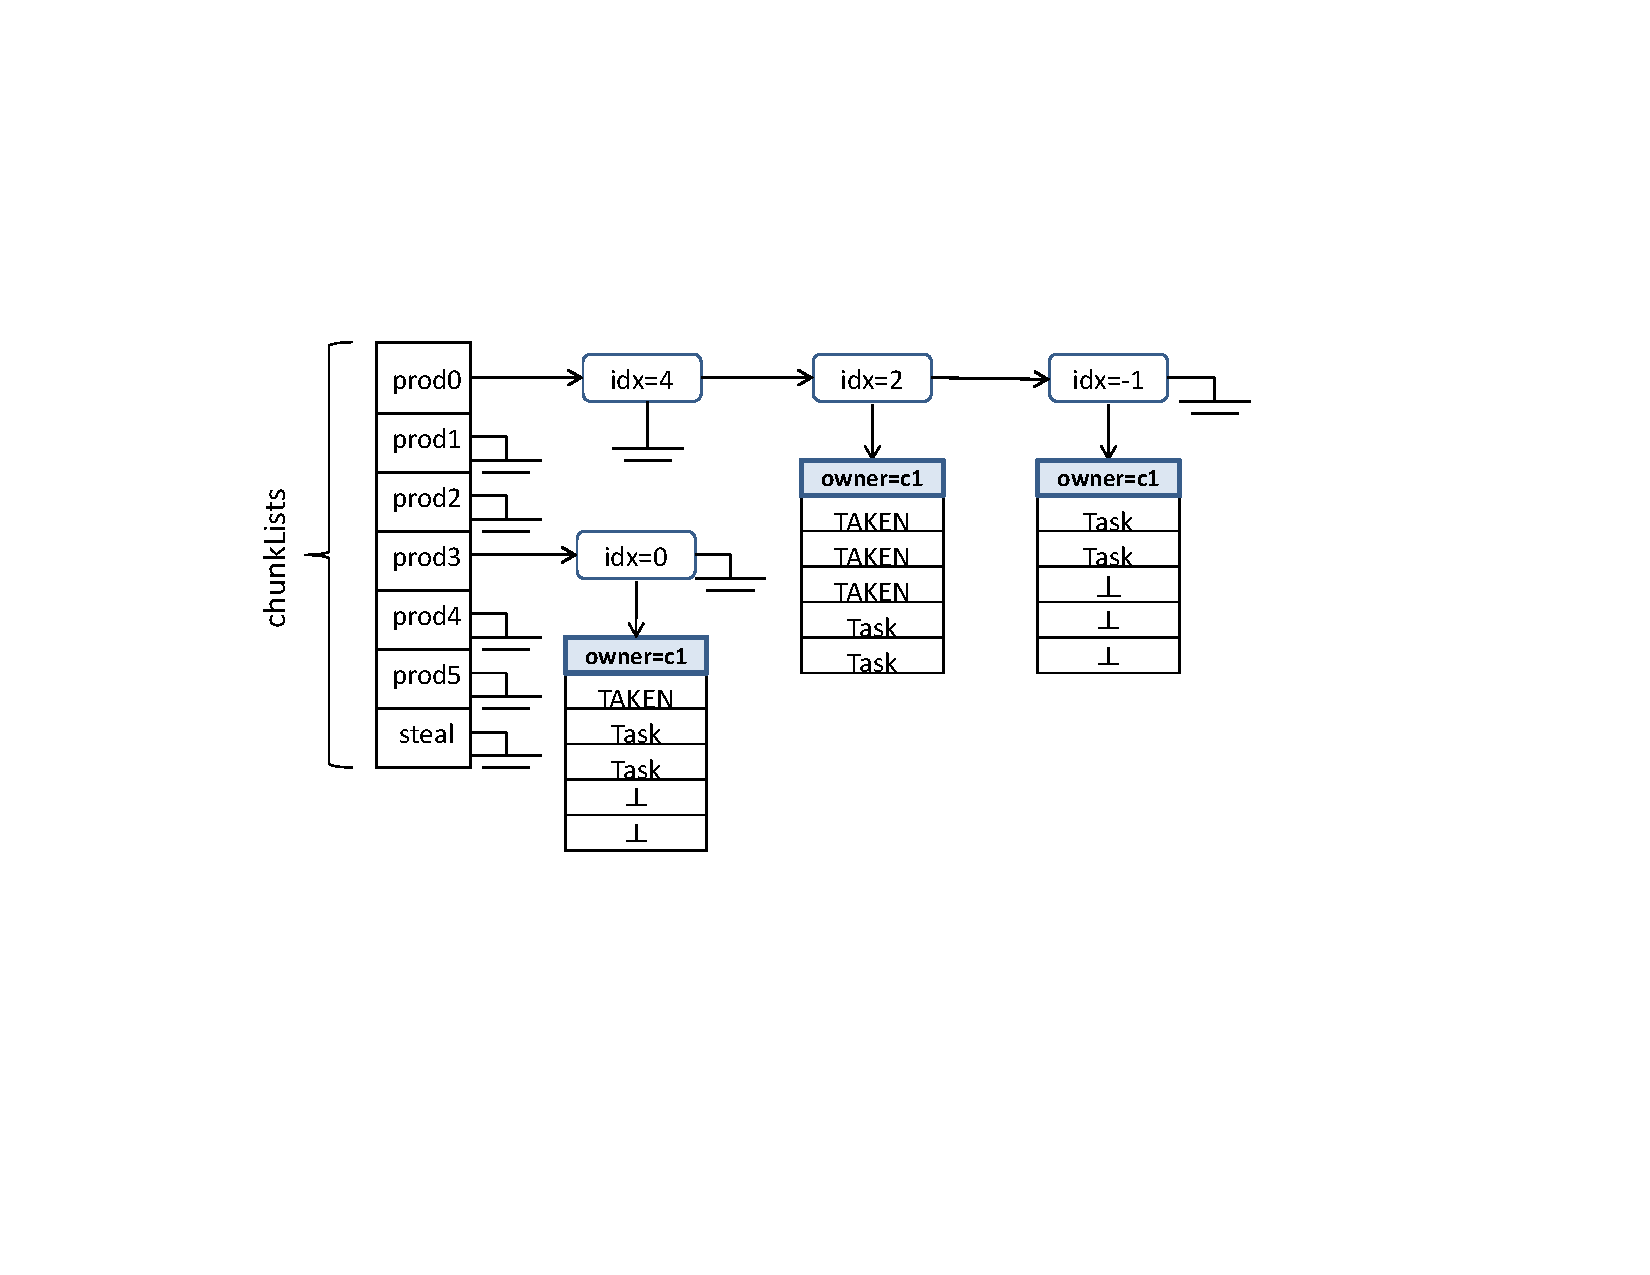
\includegraphics[height=0.3\textwidth]{figures/salsa-struct}
	\caption{
	    \footnotesize{Overview of the SALSA per-consumer pool. Each producer has a list of
nodes that points to chunks. Empty node are lazily removed. The last list is used for chunks that
the consumer stole from other SALSA pools. The index in each node indicates the location of the
next available task in the chunk and is used when stealing}}
	\label{fig:salsa-struct}
\end{figure}

In this section we describe the structure of the SALSA implementation of a single-consumer pool.
The structure is described in Algorithm~\ref{alg:non-fifo-ds} and Figure~\ref{fig:salsa-struct}

The structure is composed of number of producers + 1 lists of nodes. The first lists corresponds to
the producers, and the last list is used for stolen chunks. Each node has a pointer to a
chunk and an index (idx), this indicates the index of the last task already taken or the index of
a task which is about to be taken by the consumer, this field is used by a consumer to know what is
the next available task in the chunk and it is also used when stealing chunks (see
Section~\ref{alg-stealing}).
Chunks are arrays of pointers to tasks. When there is no task in a cell it contains $\bot$, after
the task was taken by a consumer, the cell will contain the special value \emph{TAKEN}. Each chunk
has an owner which is the ID of the consumer that is currently working with that chunk. 

The lists are single-writer multiple reader linked-lists, similar to the one shown
in~\cite{Michael:2004:HPS:987524.987595}. Producer $i$ is owner of list $i$ and the consumer is the
owner last list, the only one to modify the list is the owner. Nodes are removed lazily: when a list
owner sees a node that does not point to a chunk, this node is removed and reclaimed. When a
producer wishes to add a new chunk to the list, he traverses the list, removing nodes without chunks
while doing so, then he appends to the list a new node that points to the new chunk. Hazard
pointers~\cite{Michael:2004:HPS:987524.987595} are used to manage the reclamation of nodes and
chunks and solve the ABA problem. 

Each Consumer has a chunk pool, which is implemented using a
lock-free queue~\cite{Michael:1996:SFP:248052.248106}. These pools are used to enable reuse of
chunks, and also so producers can realize when a consumer is full and move to another consumer (see
Section~\ref{alg-pools}).
